\subsubsection{General Approach}

The chess commentator has the task of translating certain information, which it receives from the chess engine described before, into human understandable comments. Such a task falls into the domain of \textit{sequence-to-sequence} processing. The idea of sequence-to-sequence models is to map an input of a certain length to an output of a certain length, where input and output length can be different.\footnote{Cf. \cite{Sutskever-2014-sts}, p. 1} For such tasks, encoder-decoder architectures with attention has achieved great success in the past. An architecture proposed by \cite{zang-etal-2019-automated} consists of two parts, an encoder and a decoder, which are two \textit{bidirectional recurrent neural networks (Bi-RNN) using long short-term memory (LSTM) state cells}.

Recurrent neural networks (RNN) are neural networks designed to process sequences of data. RNNs process the data sequences in a time-dependent manner by putting the generated outputs back into the network along with new inputs.\footnote{Cf. \cite{rnn-2015-review}, p. 2} This allows the network to remember ongoing patterns in the data and respond to those patterns. State and time are related in recurrent networks because the reused output and the newly added input adjust the values in the RNN accordingly.\footnote{Cf. \cite{rnn-2015-review}, p. 8} The state in the network, therefore, represents the values of the neurons in the network at a given time. Bidirectional recurrent neural networks are a special type of recurrent networks that consider both the previous and subsequent input data, unlike traditional RNNs that consider only the previous input data.\footnote{Cf. \cite{https://doi.org/10.48550/arxiv.1801.01078}, p. 1} This is done by splitting "the state neurons of a regular RNN in a part that is responsible for the positive time direction (forward states) and a part for the negative time direction (backward states)"\footnote{\cite{Schuster1997BidirectionalRN}, p. 2674}. This enables them to remember and respond to ongoing patterns in both directions along the sequence. One problem of RNNs and Bi-RNNs is the processing of long input sequences, where the so-called "vanishing gradient problem" can occur, whereby the network is no longer able to correctly consider the information from the past. This can be solved by recurrent networks that use a long short-term memory architecture. LSTM cells are special neurons that allow the network to remember and respond to ongoing patterns over long periods of time.\footnote{Cf. \cite{rnn-2015-review}, p. 17} This makes them particularly well suited for processing sequences where patterns persist over an extended period of time.

\begin{figure}[h]
\centering
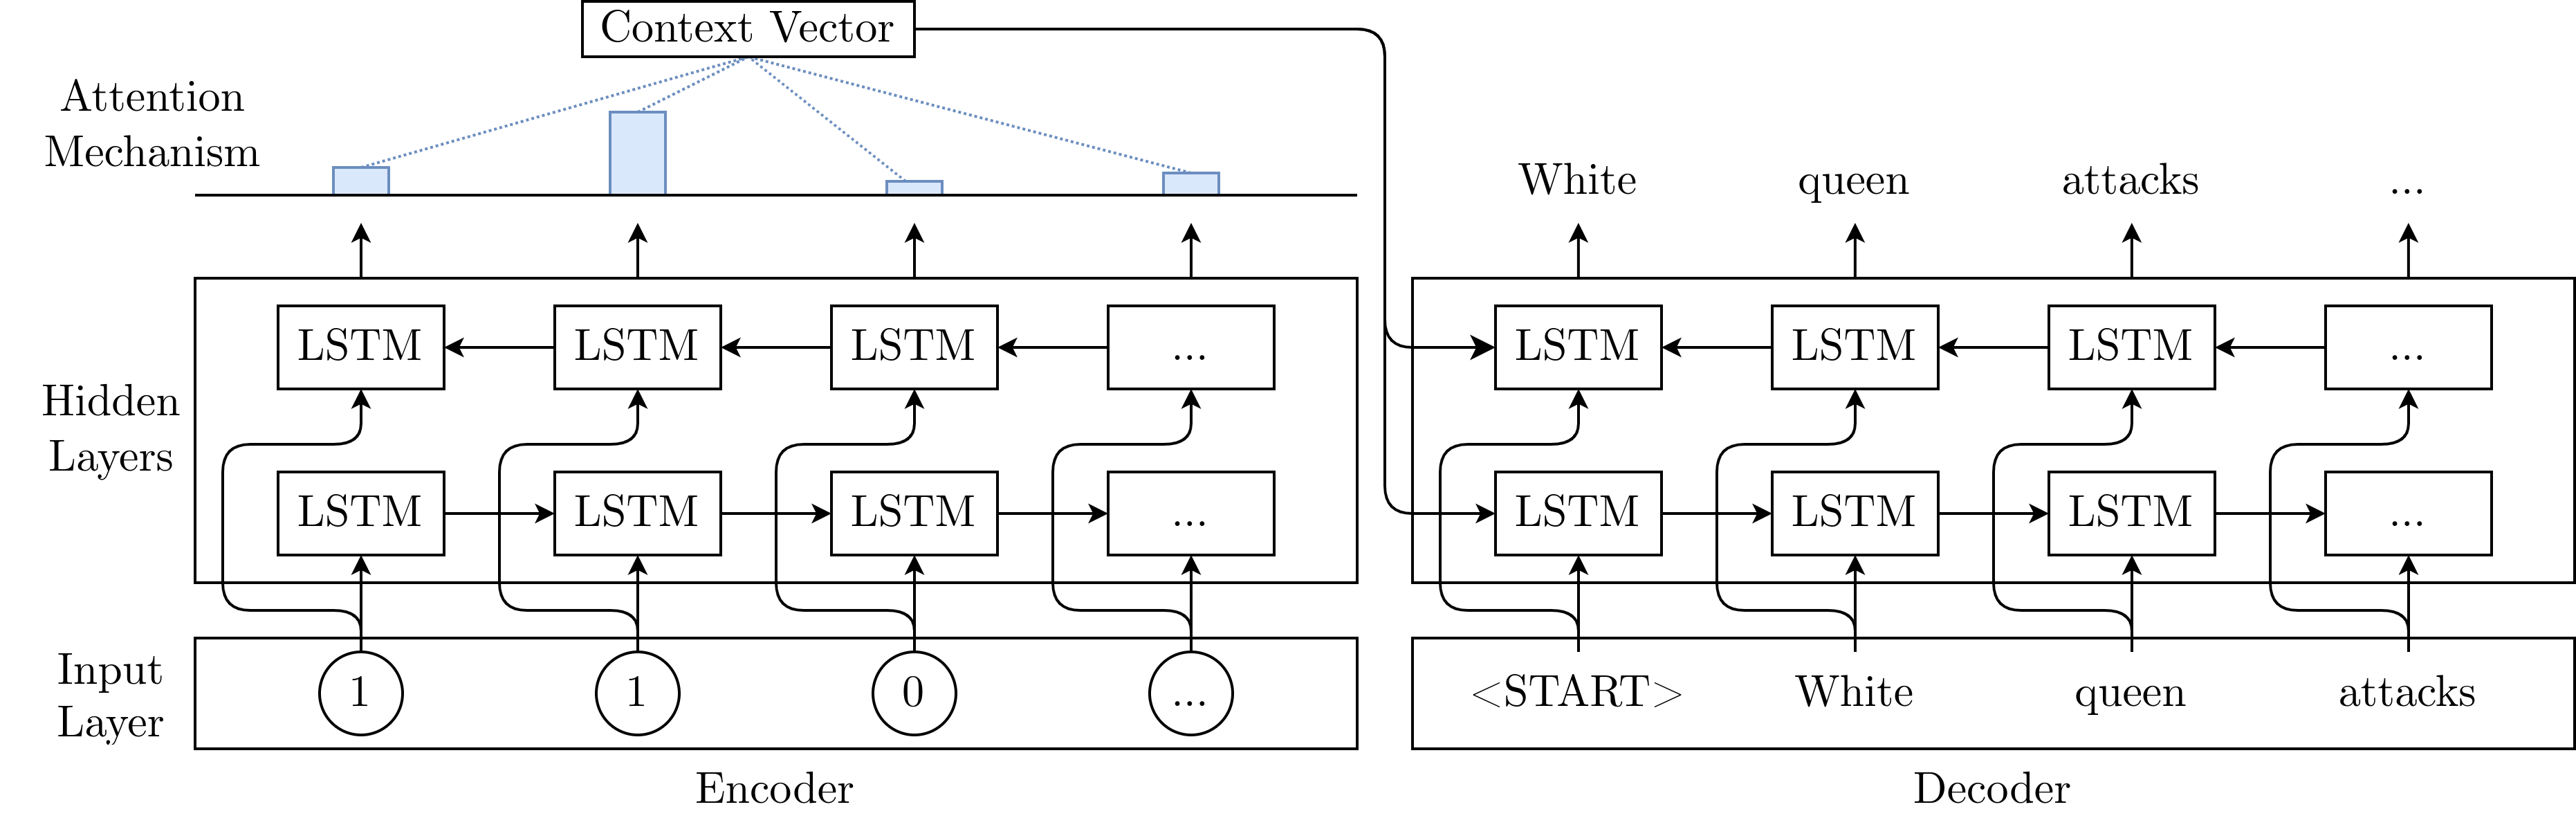
\includegraphics[width=\textwidth]{graphics/commentator_example/general_approach.png}
\caption{Chess Commentator Encoder-Decoder Architecture with Attention Mechanism (Note: Figure based on \cite{jhamtani-etal-2018-learning} Figure 4)}
\label{fig:eda}
\end{figure}

The encoder-decoder architecture used for generating chess commentary makes use of the described Bi-LSTMs.\footnote{Cf. \cite{zang-etal-2019-automated}, p. 2}  It’s a model used in machine translation and other areas of artificial intelligence. It consists of two main components: the encoder and the decoder. The encoder is responsible for converting the input into an appropriate representation (e.g., a vector of numbers). The decoder uses this representation to produce the desired output.\footnote{Cf. \cite{https://doi.org/10.48550/arxiv.1406.1078}, p. 1} In the case of the chess commentary translation the encoder receives a sequence of data, generated by the chess engine (position and move), processes the data and encodes it  into a "fixed-length vector representation"\footnote{\cite{cho-2014-ende}, p. 1}. This vector are the last states of the encoder. The vector can either be used as initialization for the LSTM cells of the decoder or as additional input for each step of the generation of the output.\footnote{Cf. \cite{mohajerin-2017-state}, pp. 1-2} One problem that affects the quality of the decoder’s translation, is the length of the sequences. The sequence stored in the vector tends to dilute over time, resulting in poor translations. To solve it, an attention mechanisms can be used. The attention mechanism allows the decoder to "selectively focusing on parts of the source"\footnote{\cite{luong-2015-attention}, p. 1} while producing the desired output. This is done while processing the data in the encoder, which encodes only the most important information in the vector, called the context vector. It can be said that the context vector contains a summary of the sequence. This allows the decoder to focus only on the information relevant for translation. If the decoder now wants to generate comments, it receives a start symbol as input (represented by \texttt{<START>} in Figure \ref{fig:eda}). This start symbol is used to indicate the start of the output sequence. The first output is the first word of the translation. The output is additionally used as new input in the next step, generates an output and which is used as the new input again. This procedure is repeated until an end symbol is reached, which signals the end of the sequence. The generated output sequence is the translation, so here the chess comments.